\section{Security in the pipeline}
Security in the pipeline ensures the code's utmost safety from various security threats. The \gls{pipeline} actively incorporates security measures and implements strict controls. The pipeline commonly consists of multiple phases like code development, testing, and deployment, all of which may be susceptible to various security threats, like unauthorized access, data breaches, malware, and \gls{denial-of-service} attacks. Therefore, security in the pipeline is crucial to secure the integrity and confidentiality of software applications and data. The \gls{pipeline} can use the following tools below to enhance its security. For examples of the specific tools, see chapter \ref{chap:Tools}. 

\subsection{Code scanning}
\label{Code Scanning}
According to Microsoft's best practices for secure \acrshort{sdlc} \cite{microsoftSDLCpractices}, a \acrshort{sast} tool should be included in the \gls{pipeline}. A \acrshort{sast} tool can be, for example, code scanning. Code scanning is a security measure that analyses code with the help of a tool to find security vulnerabilities and coding errors. Code scanning serves as a preventive measure against developers introducing new issues. In Figure \ref{fig: Pipeline with implemented SAST scan}, the \acrshort{sast} scan is set to be in GitHub \cite{sast}. By doing this scan there, it is done at the earliest stage possible, before the code is moved forward in the pipeline, eliminating vulnerabilities as soon as possible.

 \vspace{2mm}
\begin{figure}[H]
    \centering
    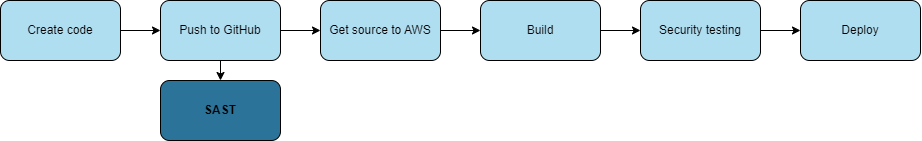
\includegraphics[width=0.8\columnwidth]{Images/pipeline2.png}
    \caption{Pipeline with implemented \acrshort{sast} scan}
    \label{fig: Pipeline with implemented SAST scan}
\end{figure}

\subsection{Scan dependencies and open source libraries}
\label{Scan Dependencies and Open Source Libraries}
Dependencies can be divided into two parts: \textit{direct} and \textit{transitive} \cite{googledependency}. A direct dependency is a directly referenced software component in an application. A transitive is a functional software component necessary for an application's direct \gls{dependency}. These \gls{dependency} may have their own set of direct and indirect \gls{dependency}, resulting in a recursive tree of transitive \gls{dependency} affecting the application. This means that the \gls{dependency} used in the code may be linked to numerous additional dependents, creating a large supply chain. To secure these supply chains, in addition to vulnerability scanning, the company can create a clear policy for evaluating and managing \gls{dependency}, including criteria for selecting secure and trustworthy libraries and frameworks. They should also limit unnecessary or outdated \gls{dependency}, as these can increase the attack surface and create unnecessary risk. 
\\~\\
All dependencies, open-source libraries, and third-party \gls{artifact}s that have been utilized should be validated \cite{bestpracticeSupplyChain}. To validate a file's integrity, compare the signature of an artifact to the signature generated by the artifact provider. This comparison helps detect any unauthorized alterations, tampering, or corruption of dependencies that may occur due to a \gls{maninthemiddle} or a compromise of the artifact repository. If any third-party software is used in the application, conducting an \acrshort{sca} scan with appropriate tools is crucial to detect any vulnerable open-source software implemented. 
\\~\\
The \acrshort{sca}  is used in conjunction with the \acrshort{sast} tool in Figure \ref{fig: Pipeline with implemented SCA scan}. Similarly to \acrshort{sast}, it is done in GitHub to patch the vulnerable \gls{dependency} early in the implementation phase. \cite{scaplasment}

\vspace{2mm}
\begin{figure}[H]
    \centering
    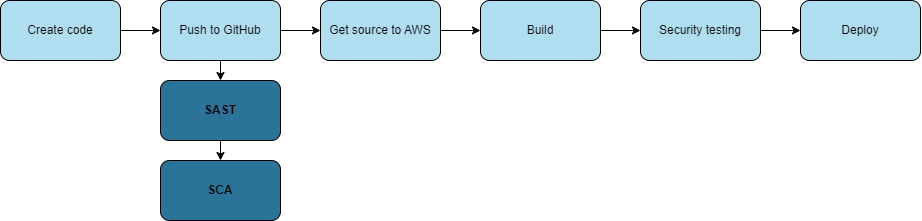
\includegraphics[width=0.8\columnwidth]{Images/pipeline3.png}
    \caption{Pipeline with implemented \acrshort{sca} scan}
    \label{fig: Pipeline with implemented SCA scan}
\end{figure}

\subsection{Secret scanning}
\label{Secret scanning}
To prevent or identify accidental exposure of \say{secrets}, like access tokens, SSH keys, or other credentials, secret scanning should be executed on the repository where the source code is stored \cite{GithubSecretScanning}. Such secrets can give unwanted access to, for example, accounts, software, or cloud providers. With access to secrets like cloud credentials, a threat actor could, among other harmful attacks, scale up the use of various costly resources, costing a company much more than what they have budgeted for \cite{GitGuardianexploitexample}. According to GitGuardian's early report on secret leaks \cite{GitGuardiansecretsprawl}, they detected 10 million secrets leaked in 2022, which is an increase of 67\% from 2021. According to the report, 1 out of every 10 GitHub authors has accidentally shared a secret in their repository, highlighting a growing problem with leaked confidential information. Developers can use secret scanning tools to search for vulnerabilities and receive alerts regarding potential security risks. 
\\~\\
In Figure \ref{fig: Pipeline with implemented secret scan}, it is recommended to perform secret scanning together with \acrshort{sast} and \acrshort{sca} for the same reason, explained in sections \ref{Code Scanning} and \ref{Scan Dependencies and Open Source Libraries}.

\vspace{2mm}
\begin{figure}[H]
    \centering
    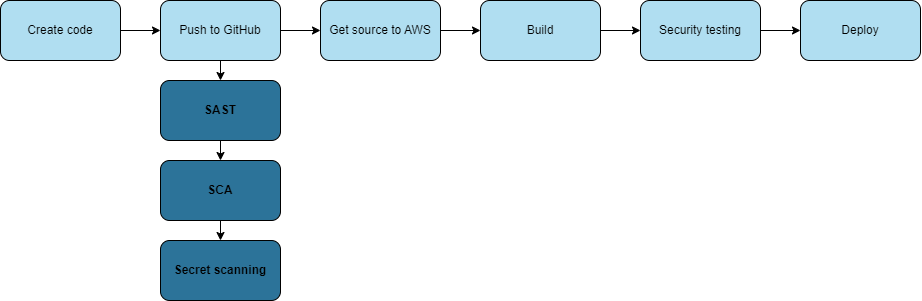
\includegraphics[width=0.8\columnwidth]{Images/pipeline4.png}
    \caption{\gls{pipeline} with implemented secret scan}
    \label{fig: Pipeline with implemented secret scan}
\end{figure}

\subsection{Dynamic scanning}
In software best practices, it is recommended to run multiple tests and scans to identify bugs and errors - where one of these tests is \acrlong{dast} (\acrshort{dast}) \cite{bestpracticeSupplyChain}. This scanning method tries to penetrate the application, attempting to identify its vulnerabilities and weaknesses. A specialized tool for \acrshort{dast} scan, such as \acrshort{owasp} \acrshort{zap}, can be implemented to identify security risks like
\gls{Cross-site scripting}, \gls{SQL-injection} or path traversal \cite{dynamictesting}.


\subsection{Manual security testing}
Even though \acrshort{dast} can be used to identify potential vulnerabilities, certain types of threats may go undetected \cite{dastpentesting}. For this reason, the company should engage a red team, a group of experts capable of performing penetration testing (pentesting). A penetration test will provide a more realistic test, as it simulates a real-world attack, detects more complex vulnerabilities, and provide a more comprehensive view of an application's security posture. In addition, a penetration test can verify the results of a  \acrshort{dast} scan by assessing whether a vulnerability can be exploited and the extent of the damage it could cause. 
\\~\\
Figure \ref{fig: Pipeline with implemented DAST scan and pentesting} shows that the \acrshort{dast} scan and penetration test are positioned later in the \gls{pipeline} because they require a running application to be executed \cite{dastplacment}. These tests cannot be performed earlier but must be conducted before the application is deployed.
\vspace{2mm}

\begin{figure}[H]
    \centering
    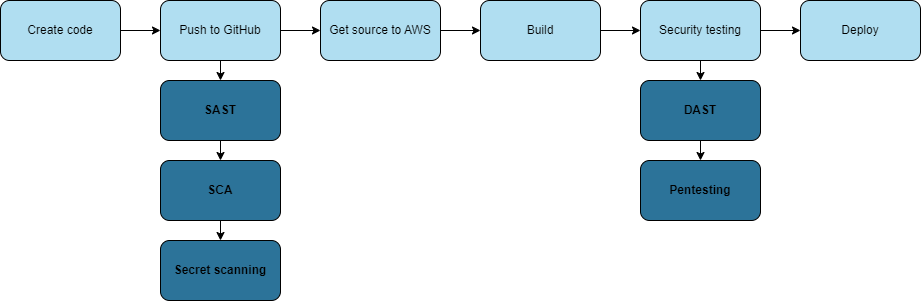
\includegraphics[width=0.8\columnwidth]{Images/pipeline5.png}
    \caption{\gls{pipeline} with implemented \acrshort{dast} scan and pentesting}
    \label{fig: Pipeline with implemented DAST scan and pentesting}
\end{figure}
